\chapter[Momento angolare e fluidi]{Il momento angolare e l'energia dei fluidi}

Nel capitolo ``I princìpi di conservazione'' abbiamo studiato la conservazione dell'energia meccanica e della quantità di moto. Restano due grandezze che, in un sistema isolato, si conservano: il \textbf{momento angolare}, che governa i moti di rotazione, e l'\textbf{energia meccanica di un liquido in movimento}, che porta all'equazione di Bernoulli. Sono l'argomento di questo capitolo, che completa la trattazione dei princìpi di conservazione.

\section[L'accelerazione angolare]{L'accelerazione angolare}

Studiando il moto circolare abbiamo introdotto la \textbf{velocità angolare} $\omega = \Delta\alpha / \Delta t$, la rapidità con cui il raggio descrive l'angolo. Se $\omega$ è costante il moto è circolare uniforme e la velocità lungo la traiettoria, la \textbf{velocità tangenziale} $v = \omega\,r$, è anch'essa costante.

Se invece il moto di rotazione \emph{non} è uniforme, sia $v$ sia $\omega$ cambiano nel tempo. La variazione della velocità tangenziale nell'unità di tempo è l'\textbf{accelerazione tangenziale} $a_t = \Delta v / \Delta t$; la variazione della velocità angolare nell'unità di tempo è l'\textbf{accelerazione angolare}.

\begin{definizione}
L'\textbf{accelerazione angolare} $\alpha$ è il rapporto fra la variazione di velocità angolare e l'intervallo di tempo in cui avviene:
\[ \colorboxed{ocre}{ \alpha = \frac{\Delta\omega}{\Delta t}. } \]
Si misura in \textbf{radianti al secondo quadrato} (\si{\radian\per\second\squared}) e rappresenta di quanto varia $\omega$ in ogni secondo.
\end{definizione}

Partendo da $v = \omega\,r$ e dividendo la variazione per $\Delta t$ si ottiene la relazione fra le due accelerazioni, analoga a $v = \omega\,r$:
\[ a_t = r\,\alpha. \]

\begin{figure}[!htbp]
    \centering
    \begin{tikzpicture}[>=stealth]
        \draw[gray,dashed] (0,0) circle (2);
        \fill (0,0) circle (1.5pt);
        \node[below left] at (0,0) {$O$};
        % raggio alla massa
        \draw (0,0) -- (35:2) node[midway,above,sloped]{\footnotesize $r$};
        \fill[ocre] (35:2) circle (2.2pt);
        \node[right] at (35:2) {$m$};
        % velocita tangenziale
        \draw[->,very thick,ocre] (35:2) -- ($(35:2)+(125:1.4)$) node[above]{$\vec v$};
        % accelerazione tangenziale
        \draw[->,very thick,red!70!black] (35:2) -- ($(35:2)+(125:0.8)$);
        \node[red!70!black,right] at ($(35:2)+(125:0.55)$) {\footnotesize $\vec a_t$};
        % verso di rotazione
        \draw[->,thick] (200:2.35) arc[start angle=200,end angle=150,radius=2.35];
        \node at (175:2.7) {$\omega$};
    \end{tikzpicture}
    \caption{Una massa $m$ che percorre una circonferenza di raggio $r$. Se il moto non è uniforme, la velocità angolare $\omega$ varia con accelerazione angolare $\alpha$, e la velocità tangenziale $\vec v$ varia con accelerazione tangenziale $\vec a_t = r\,\alpha$, diretta lungo la tangente.}
    \label{fig:acc-angolare}
\end{figure}

\begin{testexample}[\thetcbcounter \, La centrifuga]
Una centrifuga da laboratorio parte da ferma e raggiunge \SI{600}{} giri al minuto in \SI{8,0}{\second}. Qual è la sua accelerazione angolare media?

Convertiamo la velocità angolare finale in \si{\radian\per\second}:
\[ \omega = \frac{600 \cdot 2\pi}{\SI{60}{\second}} \approx \SI{62,8}{\radian\per\second}. \]
L'accelerazione angolare media è
\[ \alpha = \frac{\Delta\omega}{\Delta t} = \frac{\SI{62,8}{\radian\per\second}}{\SI{8,0}{\second}} \approx \SI{7,9}{\radian\per\second\squared}. \]
\end{testexample}

\section[Momento di inerzia]{Momento di una forza e momento di inerzia}

Applichiamo a $m$ una forza $\vec F$ tangente alla circonferenza. Per il secondo principio della dinamica essa produce un'accelerazione tangenziale $a_t$, e usando $a_t = r\,\alpha$:
\[ F = m\,a_t = m\,r\,\alpha. \]
Il \textbf{momento} di questa forza rispetto al centro $O$ (il prodotto della forza per il suo braccio $r$, introdotto studiando l'equilibrio del corpo rigido) è
\[ M = r\,F = m\,r^2\,\alpha. \]
Il momento della forza è dunque direttamente proporzionale all'accelerazione angolare; la costante di proporzionalità è il prodotto $m\,r^2$.

\begin{definizione}
Il prodotto $m\,r^2$ si chiama \textbf{momento di inerzia} $I$ della massa $m$ rispetto all'asse di rotazione:
\[ \colorboxed{ocre}{ I = m\,r^2. } \]
Si misura in \si{\kilogram\metre\squared}.
\end{definizione}

Per un sistema di più punti materiali di masse $m_1, m_2, \dots$ poste a distanze $r_1, r_2, \dots$ dall'asse, il momento di inerzia è la somma dei singoli contributi:
\[ I = m_1\,r_1^2 + m_2\,r_2^2 + \dots \]

\begin{remark}
Il momento di inerzia dipende da \emph{come sono distribuite le masse} rispetto all'asse: più le masse sono lontane dall'asse, più grande è $I$. La stessa massa, disposta in modi diversi attorno all'asse, dà momenti di inerzia diversi.
\end{remark}

\begin{figure}[!htbp]
    \centering
    \begin{tikzpicture}[>=stealth]
        % asse di rotazione
        \draw[thick] (0,-1.7) -- (0,1.7);
        \node[above] at (0,1.7) {\footnotesize asse};
        \draw[->,thick] (-0.5,1.95) arc[start angle=160,end angle=20,radius=0.5];
        % asta
        \draw[thick] (-2.6,0) -- (3.0,0);
        % masse
        \fill[ocre] (-2.6,0) circle (3pt); \node[below] at (-2.6,0) {\footnotesize $m_1$};
        \fill[ocre] (1.4,0) circle (3.5pt);  \node[below] at (1.4,0) {\footnotesize $m_2$};
        \fill[ocre] (3.0,0) circle (2.5pt); \node[below] at (3.0,0) {\footnotesize $m_3$};
        % distanze
        \draw[<->] (0,0.5) -- (-2.6,0.5) node[midway,above]{\footnotesize $r_1$};
        \draw[<->] (0,0.9) -- (1.4,0.9) node[midway,above]{\footnotesize $r_2$};
        \draw[<->] (0,1.3) -- (3.0,1.3) node[midway,above]{\footnotesize $r_3$};
    \end{tikzpicture}
    \caption{Masse distribuite rispetto a un asse di rotazione. Il momento di inerzia del sistema è $I = m_1 r_1^2 + m_2 r_2^2 + m_3 r_3^2$.}
    \label{fig:momento-inerzia}
\end{figure}

Un corpo rigido esteso (un disco, un anello, un cilindro) si può pensare come un insieme di tante piccole masse: il suo momento di inerzia è la somma dei loro contributi. Per le forme più comuni il risultato è riportato nella tabella~\ref{tab:momenti-inerzia}.

\begin{table}[!htbp]
    \centering
    \begin{tabular}{lc}
        \toprule
        corpo (massa $m$, raggio $r$), asse per il centro & $I$ \\
        \midrule
        anello sottile (o cilindro cavo a parete sottile) & $m\,r^2$ \\
        disco (o cilindro pieno) & $\tfrac{1}{2}\,m\,r^2$ \\
        sfera piena & $\tfrac{2}{5}\,m\,r^2$ \\
        \bottomrule
    \end{tabular}
    \caption{Momento di inerzia di alcuni corpi rigidi omogenei rispetto all'asse di simmetria. A parità di massa e raggio, l'anello (masse tutte al bordo) ha $I$ maggiore del disco.}
    \label{tab:momenti-inerzia}
\end{table}

Poiché per ogni piccola massa vale $M = m\,r^2\,\alpha$ e in un corpo rigido l'accelerazione angolare $\alpha$ è la stessa per tutte, sommando si ottiene
\[ \colorboxed{ocre}{ M = I\,\alpha. } \]
Questa relazione, che lega il momento delle forze applicate all'accelerazione angolare prodotta, è l'analogo per le rotazioni del secondo principio della dinamica $F = m\,a$: il momento di inerzia $I$ gioca il ruolo della massa. Come la massa misura la resistenza di un corpo a mettersi in moto di traslazione, il momento di inerzia misura la sua resistenza a mettersi in moto di rotazione.

\begin{testexample}[\thetcbcounter \, Il momento di inerzia di un disco]
Una mola a forma di disco ha massa \SI{2,5}{\kilogram} e raggio \SI{40}{\centi\metre}. Qual è il suo momento di inerzia rispetto all'asse?
\[ I = \frac{1}{2}\,m\,r^2 = \frac{1}{2} \cdot 2{,}5 \cdot (0{,}40)^2 = \SI{0,20}{\kilogram\metre\squared}. \]
Se invece della mola avessimo un anello di uguale massa e raggio, il momento di inerzia sarebbe il doppio, $\SI{0,40}{\kilogram\metre\squared}$.
\end{testexample}

\begin{testexample}[\thetcbcounter \, Quale momento per accelerare una ruota]
Una ruota ha momento di inerzia $I = \SI{0,50}{\kilogram\metre\squared}$ e, partendo da ferma, raggiunge $\omega = \SI{18}{\radian\per\second}$ in \SI{6,0}{\second}. Quale momento delle forze l'ha fatta accelerare?

L'accelerazione angolare è $\alpha = \Delta\omega/\Delta t = 18/6{,}0 = \SI{3,0}{\radian\per\second\squared}$. Quindi
\[ M = I\,\alpha = 0{,}50 \cdot 3{,}0 = \SI{1,5}{\newton\metre}. \]
\end{testexample}

\section[Il momento angolare]{Il momento angolare e la sua conservazione}

\begin{definizione}
Si chiama \textbf{momento angolare} $L$ di un corpo che ruota il prodotto del suo momento di inerzia per la sua velocità angolare:
\[ \colorboxed{ocre}{ L = I\,\omega. } \]
Si misura in \si{\kilogram\metre\squared\per\second}. È l'analogo, per le rotazioni, della quantità di moto $p = m\,v$.
\end{definizione}

\begin{testexample}[\thetcbcounter \, Il momento angolare di un disco]
Un disco con momento di inerzia $I = \SI{0,010}{\kilogram\metre\squared}$ ruota a $\omega = \SI{20}{\radian\per\second}$. Il suo momento angolare è
\[ L = I\,\omega = 0{,}010 \cdot 20 = \SI{0,20}{\kilogram\metre\squared\per\second}. \]
\end{testexample}

Per un sistema isolato il momento angolare si comporta come la quantità di moto: quando la forza risultante è nulla la quantità di moto si conserva; quando il \emph{momento} risultante delle forze esterne è nullo, si conserva il momento angolare.

\begin{definizione}
\textbf{Principio di conservazione del momento angolare.} Il momento angolare di un corpo (o di un sistema) rimane costante se è nullo il momento risultante delle forze esterne che agiscono su di esso.
\end{definizione}

La conseguenza più vistosa si ha con i corpi \textbf{non rigidi}, che possono variare il proprio momento di inerzia spostando le masse rispetto all'asse. Se $I$ diminuisce, poiché il prodotto $L = I\,\omega$ deve restare costante, la velocità angolare $\omega$ \emph{aumenta}; se $I$ aumenta, $\omega$ diminuisce.

\begin{figure}[!htbp]
    \centering
    \begin{tikzpicture}[>=stealth]
      \foreach \x/\rr/\lab/\arc in {0/1.5/{$I$ grande, $\omega$ piccola}/25, 5/0.7/{$I$ piccolo, $\omega$ grande}/55}{
        \begin{scope}[xshift=\x cm]
            \draw[gray,dashed] (0,0) circle (\rr);
            \draw[thick] (-\rr,0) -- (\rr,0);
            \fill (0,0) circle (1.5pt);
            \fill[ocre] (-\rr,0) circle (3pt);
            \fill[ocre] (\rr,0) circle (3pt);
            \draw[->,thick] (200:\rr+0.35) arc[start angle=200,end angle=200-\arc,radius=\rr+0.35];
            \node[font=\footnotesize,align=center] at (0,-\rr-0.55) {\lab};
        \end{scope}
      }
      \draw[->,thick,gray] (2.1,0) -- (3.4,0);
    \end{tikzpicture}
    \caption{Una pattinatrice che ruota chiude le braccia lungo il corpo: il momento di inerzia diminuisce e, poiché il momento angolare $L = I\,\omega$ si conserva, la velocità di rotazione aumenta. Lo stesso principio spiega gli avvitamenti dei tuffatori e la capacità di un gatto (o di un satellite) di riorientarsi.}
    \label{fig:pattinatrice}
\end{figure}

\begin{testexample}[\thetcbcounter \, La pattinatrice]
Una pattinatrice ruota su se stessa a $\omega_i = \SI{2,0}{\radian\per\second}$ con le braccia aperte, quando il suo momento di inerzia vale $I_i = \SI{4,0}{\kilogram\metre\squared}$. Chiudendo le braccia lo riduce a $I_f = \SI{1,2}{\kilogram\metre\squared}$. Con quale velocità angolare ruota adesso?

Nessun momento esterno agisce attorno all'asse verticale (l'attrito del ghiaccio è trascurabile), quindi il momento angolare si conserva:
\[ I_i\,\omega_i = I_f\,\omega_f \quad\Rightarrow\quad \omega_f = \frac{I_i\,\omega_i}{I_f} = \frac{4{,}0 \cdot 2{,}0}{1{,}2} \approx \SI{6,7}{\radian\per\second}. \]
La velocità di rotazione è più che triplicata.
\end{testexample}

\begin{testexample}[\thetcbcounter \, La giostra]
Una bambina di \SI{30}{\kilogram} è seduta sul bordo di una giostra, a \SI{3,0}{\metre} dall'asse. La giostra ha momento di inerzia $I_g = \SI{400}{\kilogram\metre\squared}$ e ruota a $\omega_i = \SI{0,52}{\radian\per\second}$. Con quale velocità angolare ruota il sistema se la bambina si sposta fino all'asse di rotazione?

Il momento di inerzia iniziale del sistema è quello della giostra più quello della bambina, vista come massa puntiforme:
\[ I_i = I_g + m\,r^2 = 400 + 30 \cdot (3{,}0)^2 = \SI{670}{\kilogram\metre\squared}. \]
Quando la bambina è sull'asse, la sua distanza è nulla e il suo contributo scompare: $I_f = \SI{400}{\kilogram\metre\squared}$. Il momento angolare si conserva:
\[ \omega_f = \frac{I_i\,\omega_i}{I_f} = \frac{670 \cdot 0{,}52}{400} \approx \SI{0,87}{\radian\per\second}. \]
\end{testexample}

\begin{esercizio}
Un anello di massa \SI{0,50}{\kilogram} e raggio \SI{20}{\centi\metre} ruota attorno al suo asse. Qual è il suo momento di inerzia? ($I = m\,r^2$ per l'anello)\\
\risp{$I = 0{,}50 \cdot (0{,}20)^2 = \SI{0,020}{\kilogram\metre\squared}$}
\end{esercizio}

\begin{esercizio}
Una mola a disco di \SI{3,0}{\kilogram} e raggio \SI{15}{\centi\metre} ruota a \SI{40}{\radian\per\second}. Calcola il momento di inerzia e il momento angolare.\\
\risp{$I = \tfrac12 \cdot 3{,}0 \cdot (0{,}15)^2 \approx \SI{0,034}{\kilogram\metre\squared}$; \; $L = I\,\omega \approx \SI{1,4}{\kilogram\metre\squared\per\second}$}
\end{esercizio}

\begin{esercizio}
Una giostra parte da ferma e raggiunge \SI{3,0}{\radian\per\second} in \SI{5,0}{\second}. Qual è la sua accelerazione angolare media?\\
\risp{$\alpha = \dfrac{\SI{3,0}{\radian\per\second}}{\SI{5,0}{\second}} = \SI{0,60}{\radian\per\second\squared}$}
\end{esercizio}

\begin{esercizio}
Un volano ha momento di inerzia \SI{0,18}{\kilogram\metre\squared} e ruota a \SI{120}{\radian\per\second}. Qual è il suo momento angolare? Se l'attrito lo ferma in \SI{30}{\second}, qual è l'accelerazione angolare media?\\
\risp{$L = 0{,}18 \cdot 120 \approx \SI{22}{\kilogram\metre\squared\per\second}$; \; $\alpha = -120/30 = \SI{-4,0}{\radian\per\second\squared}$}
\end{esercizio}

\begin{esercizio}
Una piattaforma girevole ha momento di inerzia \SI{5,0}{\kilogram\metre\squared} e ruota a \SI{3,0}{\radian\per\second} con una persona ferma al centro. La persona si sposta verso il bordo e il momento di inerzia del sistema sale a \SI{8,0}{\kilogram\metre\squared}. Qual è la nuova velocità angolare?\\
\risp{$\omega_f = \dfrac{5{,}0 \cdot 3{,}0}{8{,}0} \approx \SI{1,9}{\radian\per\second}$ (rallenta)}
\end{esercizio}

\begin{esercizio}
Perché un tuffatore che vuole ruotare più velocemente in aria si raggomitola?\\
\risp{raccogliendo il corpo verso il baricentro riduce il momento di inerzia; poiché il momento angolare $L = I\,\omega$ si conserva (in aria nessun momento esterno agisce), la velocità angolare $\omega$ aumenta}
\end{esercizio}

\begin{esercizio}
Un CD (disco) di massa \SI{15}{\gram} e diametro \SI{12}{\centi\metre} gira a \SI{500}{} giri al minuto. Calcola il suo momento angolare. ($I = \tfrac12 m\,r^2$)\\
\risp{$I = \tfrac12 \cdot 0{,}015 \cdot (0{,}060)^2 \approx \SI{2,7e-5}{\kilogram\metre\squared}$; \; $\omega = 500 \cdot 2\pi/60 \approx \SI{52,4}{\radian\per\second}$; \; $L = I\,\omega \approx \SI{1,4e-3}{\kilogram\metre\squared\per\second}$}
\end{esercizio}

\section[La portata]{La portata di un liquido}

Passiamo ai liquidi in movimento. Consideriamo un liquido che scorre con velocità $v$ dentro un tubo di sezione costante $A$ (figura~\ref{fig:portata}). In un intervallo di tempo $\Delta t$ ogni particella avanza di un tratto $v\,\Delta t$: attraverso la sezione $A$ passa quindi un cilindro di liquido di volume $V = A \cdot v\,\Delta t$.

\begin{definizione}
Si chiama \textbf{portata} $Q$ di un liquido il volume che attraversa una sezione del tubo nell'unità di tempo:
\[ \colorboxed{ocre}{ Q = \frac{V}{\Delta t} = A\,v. } \]
Nel Sistema Internazionale si misura in \si{\metre\cubed\per\second}. Nell'uso pratico è comune anche il litro al secondo (\si{\litre\per\second}).
\end{definizione}

\begin{figure}[!htbp]
    \centering
    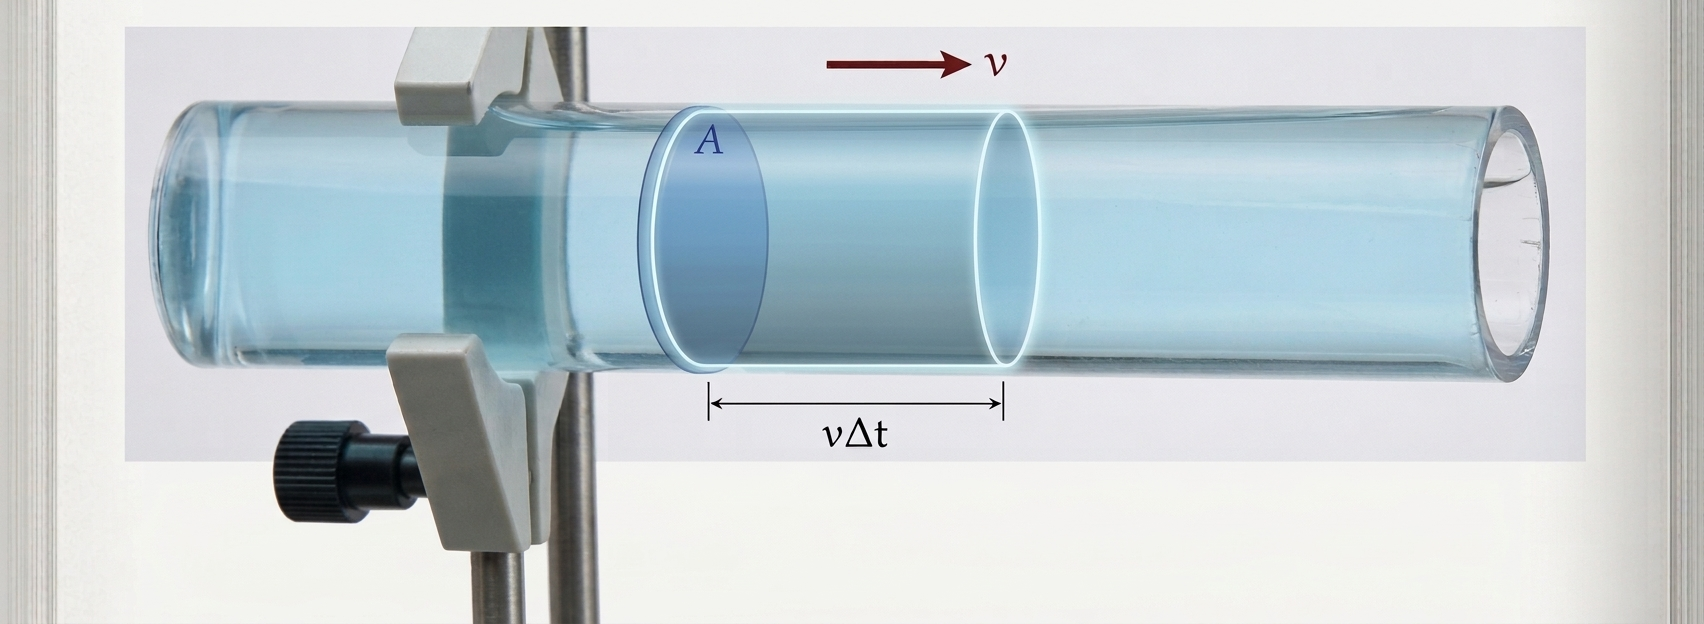
\includegraphics[width=0.92\linewidth]{img/portata-tubo.jpg}
    \caption{In un tempo $\Delta t$ attraverso la sezione $A$ passa un cilindro di liquido lungo $v\,\Delta t$. La portata è $Q = A\,v$.}
    \label{fig:portata}
\end{figure}

\begin{testexample}[\thetcbcounter \, La portata di un rubinetto]
Da un rubinetto di sezione $A = \SI{1,2}{\centi\metre\squared}$ l'acqua esce a $v = \SI{1,5}{\metre\per\second}$. Qual è la portata? Quanti litri escono in un minuto?

Conviene lavorare in unità SI: $A = \SI{1,2e-4}{\metre\squared}$.
\[ Q = A\,v = \SI{1,2e-4}{} \cdot 1{,}5 = \SI{1,8e-4}{\metre\cubed\per\second} = \SI{0,18}{\litre\per\second}. \]
In un minuto: $0{,}18 \cdot 60 \approx \SI{11}{\litre}$.
\end{testexample}

\section[L'equazione di continuità]{L'equazione di continuità}

Consideriamo ora un tubo con due sezioni $A_1$ e $A_2$ di area diversa (figura~\ref{fig:continuita}), in cui il liquido scorre con velocità $v_1$ e $v_2$. I liquidi sono \textbf{incomprimibili}: la quantità di liquido che entra da una parte nell'unità di tempo deve uscire dall'altra. La portata è quindi la stessa nelle due sezioni.

\begin{definizione}
\textbf{Equazione di continuità.} In un tubo percorso da un liquido incomprimibile la portata è costante:
\[ \colorboxed{ocre}{ A_1\,v_1 = A_2\,v_2. } \]
\end{definizione}

Ne segue che $A$ e $v$ sono \textbf{inversamente proporzionali}: dove il tubo si restringe, il liquido accelera; dove si allarga, rallenta. È l'effetto che si sfrutta stringendo con un dito l'estremità di una canna dell'acqua per far arrivare il getto più lontano.

\begin{figure}[!htbp]
    \centering
    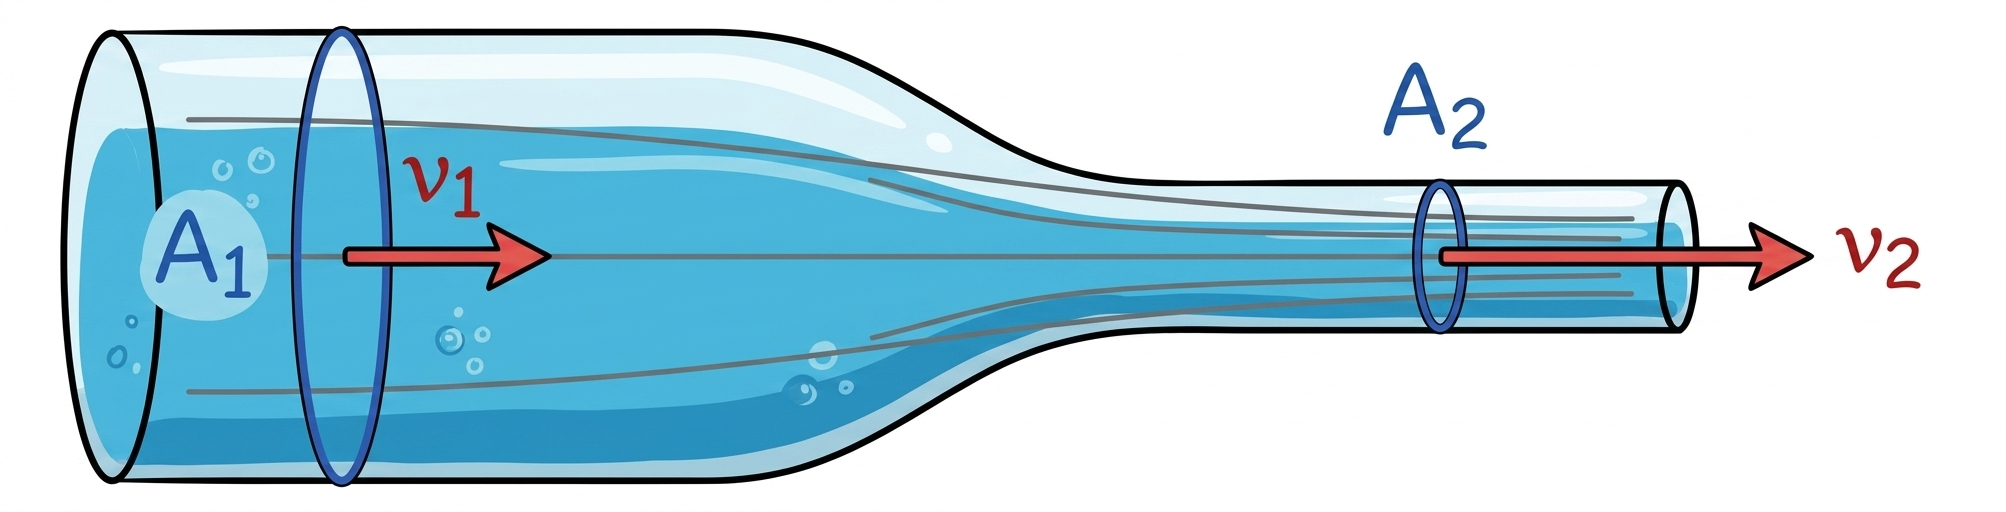
\includegraphics[width=\linewidth]{img/continuita.jpg}
    \caption{Tubo a sezione variabile. Dove la sezione è minore ($A_2 < A_1$) la velocità è maggiore ($v_2 > v_1$): le linee di flusso si addensano.}
    \label{fig:continuita}
\end{figure}

\section[L'equazione di Bernoulli]{L'equazione di Bernoulli}

Consideriamo un tubo \textbf{inclinato}, in cui cambiano sia la sezione sia la quota (figura~\ref{fig:bernoulli}). Nell'intervallo $\Delta t$ una certa massa di liquido viene sollevata dalla quota $h_1$ alla quota $h_2$: la sua energia potenziale gravitazionale aumenta. Nello stesso tempo, se il tubo si restringe, la velocità aumenta e con essa l'energia cinetica.

Sia l'energia potenziale sia quella cinetica aumentano: sembra violato il principio di conservazione dell'energia meccanica. In realtà occorre tenere conto anche dell'energia legata alla \textbf{pressione} del liquido. Pensiamo a un palloncino pieno d'acqua: se lo schiacciamo, l'acqua schizza fuori con energia cinetica. Nei liquidi la pressione è una forma di ``accumulo'' di energia.

\begin{figure}[!htbp]
    \centering
    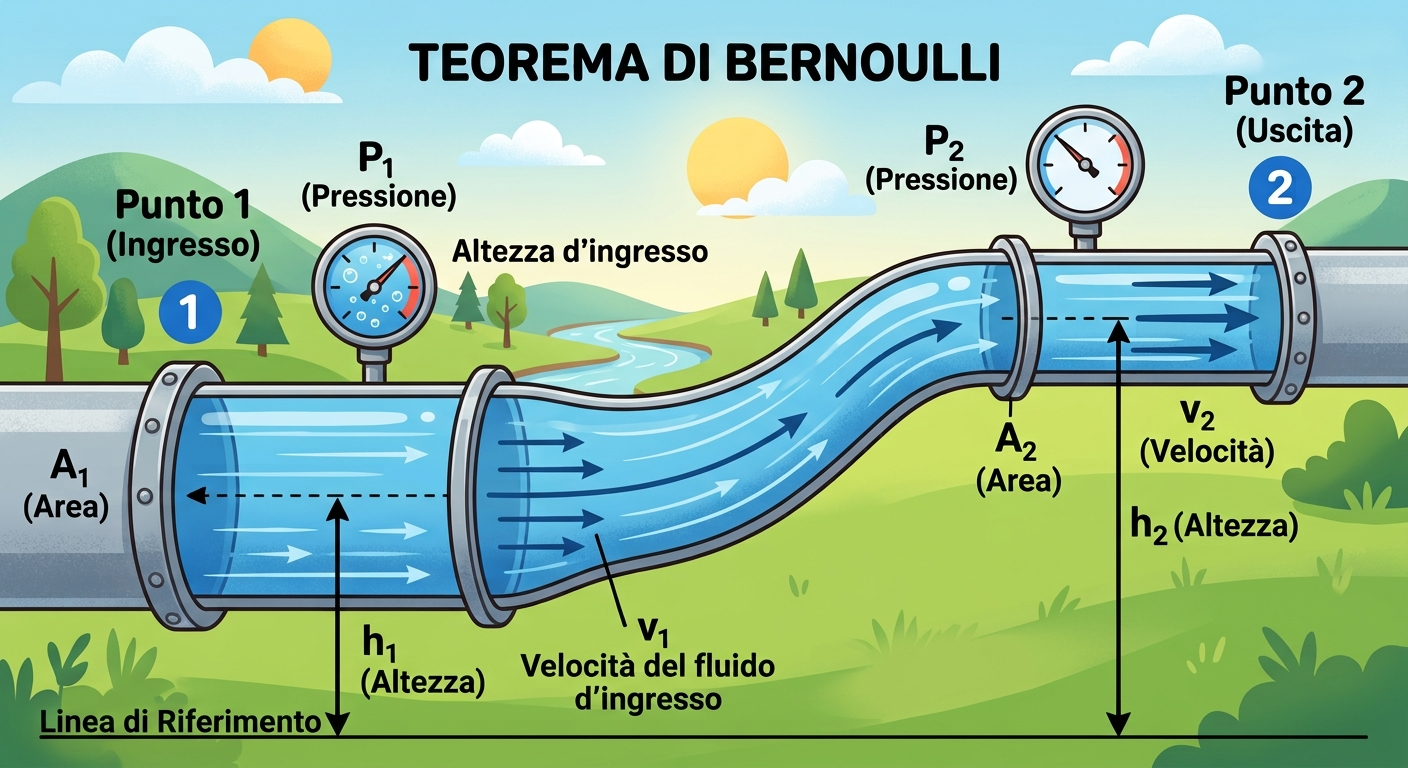
\includegraphics[width=0.95\linewidth]{img/bernoulli-tubo.jpg}
    \caption{Flusso in un tubo che sale e si restringe: dal punto 1 (ingresso, sezione $A_1$, quota $h_1$) al punto 2 (uscita, sezione $A_2 < A_1$, quota $h_2 > h_1$) aumentano sia la quota sia la velocità. L'aumento di energia potenziale e cinetica è compensato da una diminuzione di pressione ($p_2 < p_1$), misurabile con i manometri.}
    \label{fig:bernoulli}
\end{figure}

Prendendo due sezioni qualsiasi del flusso e detta $d$ la densità del liquido, il bilancio dell'energia meccanica per unità di volume si scrive:
\[ p_1 + d\,g\,h_1 + \frac{1}{2}\,d\,v_1^2 = p_2 + d\,g\,h_2 + \frac{1}{2}\,d\,v_2^2. \]

\begin{definizione}
\textbf{Equazione di Bernoulli.} Per un liquido ideale (privo di viscosità e attriti interni) che scorre in un tubo, la somma della pressione, dell'energia potenziale gravitazionale e dell'energia cinetica per unità di volume è costante:
\[ \colorboxed{ocre}{ p + d\,g\,h + \frac{1}{2}\,d\,v^2 = \text{costante}. } \]
Qui $p$ è la pressione (\si{\pascal}), $d$ la densità (\si{\kilogram\per\metre\cubed}), $h$ la quota rispetto a un livello di riferimento e $v$ la velocità del liquido.
\end{definizione}

L'equazione di Bernoulli è l'applicazione del principio di conservazione dell'energia meccanica al flusso di un liquido. Vale solo se il liquido è privo di attriti interni: la viscosità e la turbolenza, come l'attrito nella meccanica, dissipano energia.

\subsection{Due casi particolari}

\textbf{Tubo orizzontale.} Se non ci sono dislivelli ($h_1 = h_2$) il termine $d\,g\,h$ si semplifica e resta
\[ p + \frac{1}{2}\,d\,v^2 = \text{costante}. \]
Dove il tubo si restringe la velocità aumenta (continuità) e quindi la pressione \emph{diminuisce}. Questo risultato è chiamato \textbf{effetto Venturi}: \emph{dove un liquido scorre più veloce, la sua pressione è minore} (figura~\ref{fig:venturi}). Lo stesso vale per l'aria: è per l'effetto Venturi che un vento molto forte, scorrendo veloce sopra un tetto, vi genera sopra una depressione che può sollevarlo.

\begin{figure}[!htbp]
    \centering
    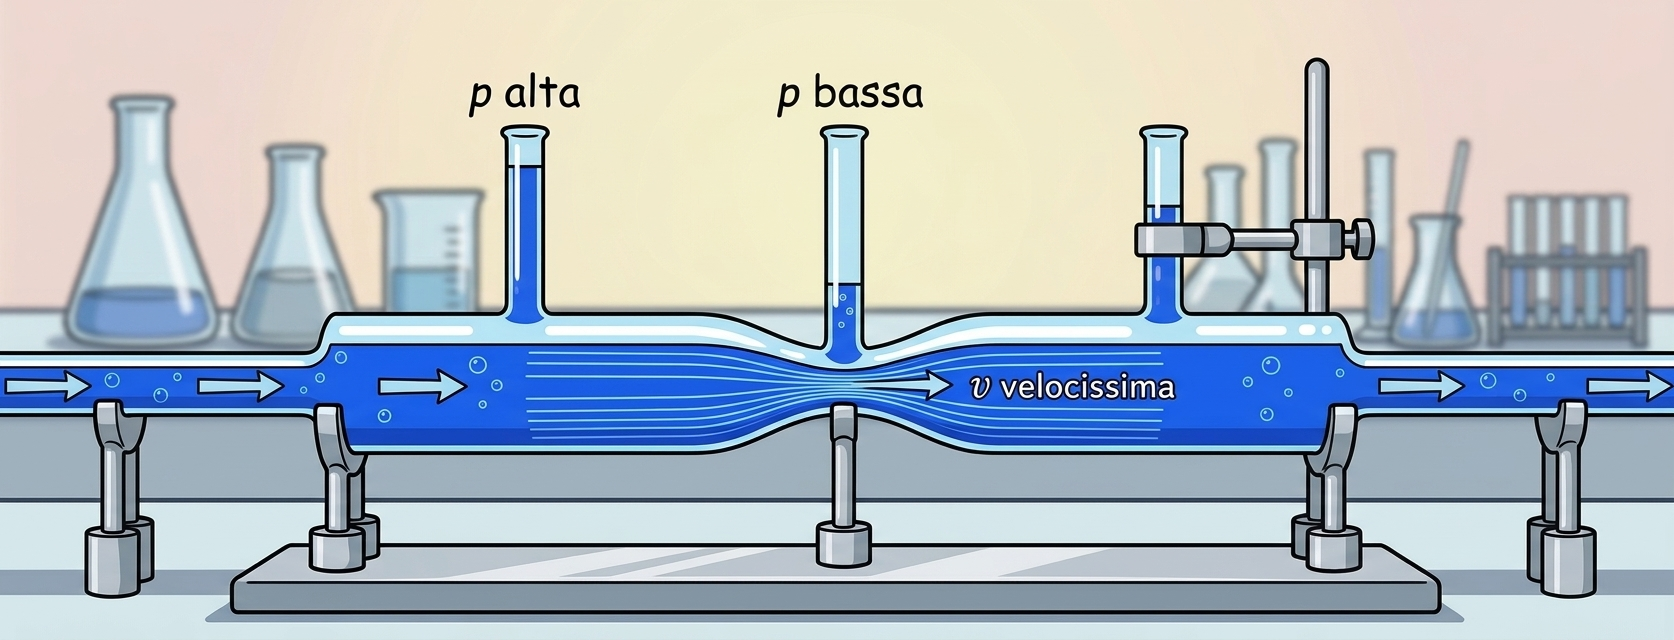
\includegraphics[width=0.95\linewidth]{img/venturi.jpg}
    \caption{Effetto Venturi. Nel tratto stretto il liquido scorre più veloce e la sua pressione è minore: il livello nel tubicino manometrico sulla strozzatura ($p$ bassa) è più basso che negli altri due.}
    \label{fig:venturi}
\end{figure}

\textbf{Tubo a sezione costante.} Se la sezione non cambia, per la continuità la velocità è costante e nell'equazione di Bernoulli scompare il termine $\tfrac12 d\,v^2$:
\[ p + d\,g\,h = \text{costante}. \]
Si ritrova la legge di Stevino: nel liquido in moto la pressione diminuisce salendo e aumenta scendendo, esattamente come nel liquido fermo.

\subsection{La legge di Torricelli}

Applichiamo l'equazione di Bernoulli a un serbatoio aperto, pieno di liquido fino a un'altezza $h$ sopra un forellino praticato sul fondo (figura~\ref{fig:efflusso-serbatoio}). Sulla superficie libera (punto 1) e all'uscita del foro (punto 2) la pressione è quella atmosferica; la superficie si abbassa molto lentamente, quindi $v_1 \approx 0$. Prendendo il foro come livello di riferimento ($h_2 = 0$, $h_1 = h$):
\[ p_\text{atm} + d\,g\,h + 0 = p_\text{atm} + 0 + \frac{1}{2}\,d\,v_2^2, \]
da cui, semplificando $p_\text{atm}$ e la densità:
\[ \colorboxed{ocre}{ v = \sqrt{2\,g\,h}. } \]

\begin{remark}
È la \textbf{legge di Torricelli}: il liquido esce dal foro con la stessa velocità che avrebbe raggiunto cadendo liberamente da un'altezza $h$. Man mano che il serbatoio si svuota $h$ diminuisce, e con essa la velocità del getto.
\end{remark}

\begin{figure}[!htbp]
    \centering
    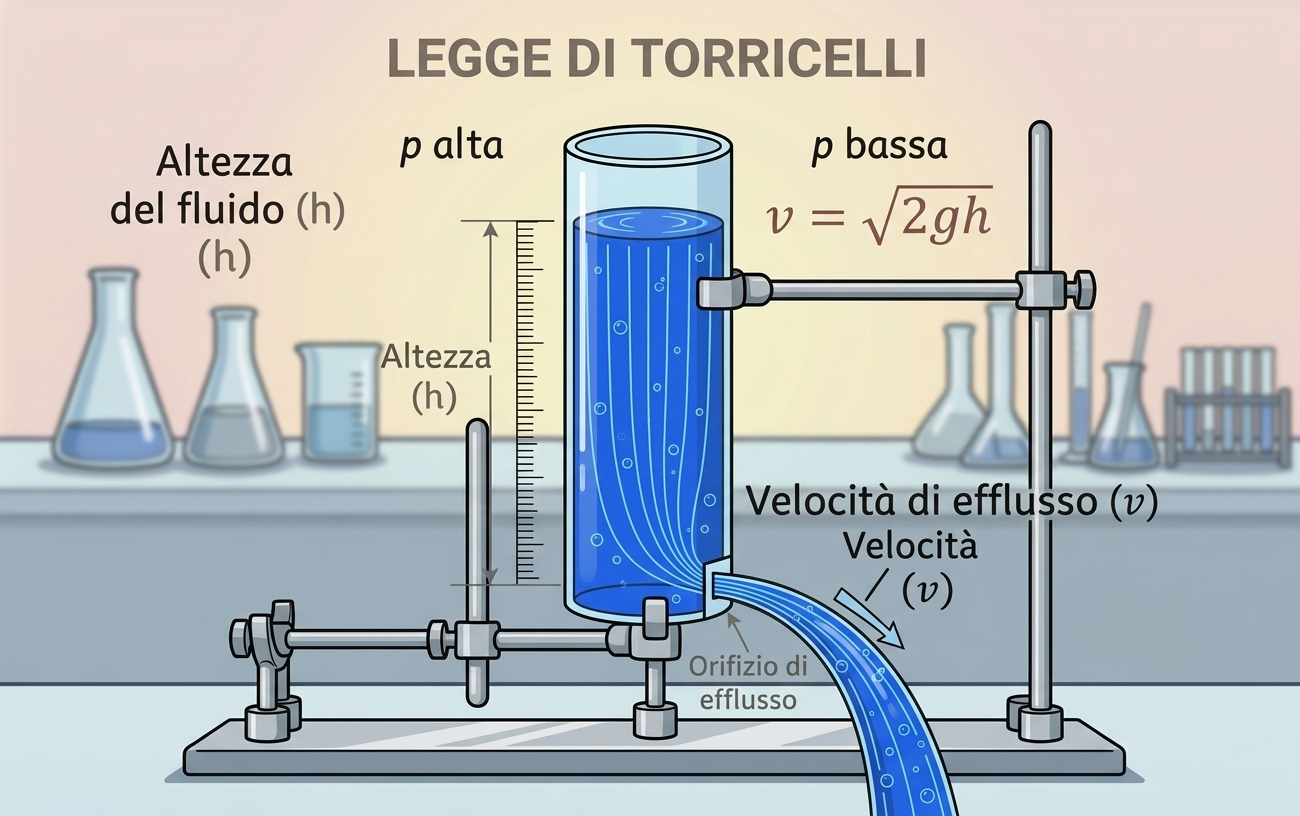
\includegraphics[width=0.72\linewidth]{img/torricelli.jpg}
    \caption{Efflusso da un serbatoio: il liquido esce dall'orifizio con velocità $v = \sqrt{2\,g\,h}$, dove $h$ è l'altezza del pelo libero sopra il foro.}
    \label{fig:efflusso-serbatoio}
\end{figure}

\begin{testexample}[\thetcbcounter \, L'ugello della canna]
In una canna dell'acqua di diametro \SI{2,0}{\centi\metre} l'acqua scorre a \SI{1,0}{\metre\per\second}. All'estremità c'è un ugello di diametro \SI{0,80}{\centi\metre}. Con quale velocità esce l'acqua?

Per l'equazione di continuità $A_1\,v_1 = A_2\,v_2$, e poiché l'area è proporzionale al quadrato del diametro:
\[ v_2 = v_1\,\frac{A_1}{A_2} = v_1 \left(\frac{d_1}{d_2}\right)^2 = 1{,}0 \cdot \left(\frac{2{,}0}{0{,}80}\right)^2 = 1{,}0 \cdot 6{,}25 \approx \SI{6,3}{\metre\per\second}. \]
\end{testexample}

\begin{testexample}[\thetcbcounter \, L'effetto Venturi]
In un tubo orizzontale scorre acqua ($d = \SI{1000}{\kilogram\per\metre\cubed}$). Nel tratto largo la velocità è $v_1 = \SI{2,0}{\metre\per\second}$ e la pressione $p_1 = \SI{1,8e5}{\pascal}$. Nel tratto stretto la sezione è la metà. Calcola la velocità e la pressione nel tratto stretto.

Dalla continuità, dimezzando la sezione la velocità raddoppia: $v_2 = \SI{4,0}{\metre\per\second}$. Dall'equazione di Bernoulli per un tubo orizzontale:
\[ p_2 = p_1 + \frac{1}{2}\,d\,(v_1^2 - v_2^2) = \SI{1,8e5}{} + \frac{1}{2} \cdot 1000 \cdot (4{,}0 - 16) \approx \SI{1,74e5}{\pascal}. \]
La pressione nel tratto veloce è minore, come previsto.
\end{testexample}

\begin{testexample}[\thetcbcounter \, Efflusso da un serbatoio]
Un serbatoio contiene acqua fino a un'altezza di \SI{10}{\metre} sopra un rubinetto posto sul fondo. Con quale velocità esce l'acqua all'apertura del rubinetto?
\[ v = \sqrt{2\,g\,h} = \sqrt{2 \cdot 9{,}81 \cdot 10} \approx \SI{14}{\metre\per\second}. \]
\end{testexample}

\begin{testexample}[\thetcbcounter \, La pompa]
Una pompa al piano terra (quota $h_1 = 0$) manda l'acqua in un tubo con pressione $p_1 = \SI{1,5}{\bar}$ e velocità $v_1 = \SI{0,80}{\metre\per\second}$. L'acqua sale fino alla quota $h_2 = \SI{3,0}{\metre}$, in un tratto di tubo di sezione dimezzata. Qual è la pressione a quella quota? ($d = \SI{1000}{\kilogram\per\metre\cubed}$)

Prima la velocità, dalla continuità (sezione dimezzata $\Rightarrow$ velocità doppia): $v_2 = \SI{1,6}{\metre\per\second}$. Poi Bernoulli, con $p_1 = \SI{1,5e5}{\pascal}$:
\[ p_2 = p_1 + d\,g\,(h_1 - h_2) + \frac{1}{2}\,d\,(v_1^2 - v_2^2). \]
\[ p_2 = \SI{1,5e5}{} + 1000 \cdot 9{,}81 \cdot (-3{,}0) + 500 \cdot (0{,}64 - 2{,}56) \approx \SI{1,2e5}{\pascal} = \SI{120}{\kilo\pascal}. \]
La pressione è calata: una parte dell'energia è servita a sollevare l'acqua e ad accelerarla.
\end{testexample}

\begin{esercizio}
Un fiume ha sezione \SI{340}{\metre\squared} e l'acqua vi scorre a \SI{0,85}{\metre\per\second}. Qual è la portata?\\
\risp{$Q = A\,v = 340 \cdot 0{,}85 \approx \SI{290}{\metre\cubed\per\second}$}
\end{esercizio}

\begin{esercizio}
Un impianto di irrigazione ha portata \SI{5,0}{\litre\per\second} e il tubo che porta l'acqua ha diametro \SI{20}{\milli\metre}. Con quale velocità scorre l'acqua nel tubo?\\
\risp{$A = \pi\,(0{,}010)^2 \approx \SI{3,1e-4}{\metre\squared}$; \; $v = Q/A = \SI{5,0e-3}{}/\SI{3,1e-4}{} \approx \SI{16}{\metre\per\second}$}
\end{esercizio}

\begin{esercizio}
In un tubo orizzontale a sezione costante scorre acqua a \SI{3,0}{\metre\per\second} con pressione \SI{2,0e5}{\pascal}. Il tubo poi sale di \SI{1,5}{\metre} mantenendo la stessa sezione. Qual è la pressione nella parte alta? ($d = 1000$, $g = 9{,}81$, in unità SI)\\
\risp{sezione costante $\Rightarrow$ $v$ costante; $p_2 = p_1 - d\,g\,\Delta h = \SI{2,0e5}{} - 1000 \cdot 9{,}81 \cdot 1{,}5 \approx \SI{1,85e5}{\pascal}$}
\end{esercizio}

\begin{esercizio}
Da un foro alla base di una diga l'acqua esce a \SI{20}{\metre\per\second}. A quale profondità sotto il pelo libero si trova il foro?\\
\risp{$h = \dfrac{v^2}{2\,g} = \dfrac{20^2}{2 \cdot 9{,}81} \approx \SI{20}{\metre}$}
\end{esercizio}

\begin{esercizio}
Un tubo passa da diametro \SI{6,0}{\centi\metre} a diametro \SI{3,0}{\centi\metre}. Se nella parte larga l'acqua scorre a \SI{1,0}{\metre\per\second}, a quale velocità scorre nella parte stretta?\\
\risp{$v_2 = v_1\,(d_1/d_2)^2 = 1{,}0 \cdot (6{,}0/3{,}0)^2 = \SI{4,0}{\metre\per\second}$}
\end{esercizio}

\begin{esercizio}
Perché il tetto di una casa può essere scoperchiato da un vento molto forte, che soffia parallelo al tetto?\\
\risp{l'aria che scorre veloce sopra il tetto ha pressione minore (effetto Venturi); l'aria quasi ferma sotto il tetto ha pressione maggiore. La differenza di pressione genera una spinta verso l'alto}
\end{esercizio}

\begin{esercizio}
Un serbatoio è pieno d'acqua fino a \SI{5,0}{\metre} sopra un forellino. Con quale velocità esce l'acqua? E quando il livello è sceso a \SI{1,25}{\metre}?\\
\risp{$v = \sqrt{2 \cdot 9{,}81 \cdot 5{,}0} \approx \SI{9,9}{\metre\per\second}$; \; con $h = \SI{1,25}{\metre}$ (un quarto), $v \approx \SI{5,0}{\metre\per\second}$ (dimezzata)}
\end{esercizio}

\section{Problemi di riepilogo}

\begin{esercizio}
Un anello di raggio \SI{0,30}{\metre} e massa \SI{1,2}{\kilogram} ruota attorno al suo asse. Qual è il momento di inerzia?\\
\risp{$I = m\,r^2 = 1{,}2 \cdot (0{,}30)^2 \approx \SI{0,11}{\kilogram\metre\squared}$}
\end{esercizio}

\begin{esercizio}
Un disco di massa \SI{4,0}{\kilogram} e raggio \SI{0,25}{\metre} ruota a \SI{30}{\radian\per\second}. Calcola il momento di inerzia e il momento angolare.\\
\risp{$I = \tfrac12 \cdot 4{,}0 \cdot (0{,}25)^2 = \SI{0,125}{\kilogram\metre\squared}$; \; $L = I\,\omega \approx \SI{3,8}{\kilogram\metre\squared\per\second}$}
\end{esercizio}

\begin{esercizio}
Una ruota con momento di inerzia \SI{0,50}{\kilogram\metre\squared} parte da ferma e raggiunge \SI{18}{\radian\per\second} in \SI{6,0}{\second}. Qual è l'accelerazione angolare media? Quale momento delle forze l'ha prodotta?\\
\risp{$\alpha = 18/6{,}0 = \SI{3,0}{\radian\per\second\squared}$; \; $M = I\,\alpha = 0{,}50 \cdot 3{,}0 = \SI{1,5}{\newton\metre}$}
\end{esercizio}

\begin{esercizio}
Due masse di \SI{2,0}{\kilogram} ciascuna sono fissate agli estremi di un'asta leggera e ruotano attorno all'asse centrale; ognuna dista \SI{0,60}{\metre} dall'asse. Qual è il momento di inerzia del sistema?\\
\risp{$I = 2 \cdot m\,r^2 = 2 \cdot 2{,}0 \cdot (0{,}60)^2 \approx \SI{1,4}{\kilogram\metre\squared}$}
\end{esercizio}

\begin{esercizio}
Una piattaforma girevole con un bambino sul bordo ha momento di inerzia \SI{10}{\kilogram\metre\squared} e ruota a \SI{2,0}{\radian\per\second}. Il bambino si sposta al centro e il momento di inerzia scende a \SI{4,0}{\kilogram\metre\squared}. Qual è la nuova velocità angolare?\\
\risp{$\omega_f = \dfrac{10 \cdot 2{,}0}{4{,}0} = \SI{5,0}{\radian\per\second}$}
\end{esercizio}

\begin{esercizio}
Un tuffatore lascia il trampolino ruotando a \SI{4,0}{\radian\per\second} con il corpo teso ($I = \SI{6,0}{\kilogram\metre\squared}$). Si raggomitola fino a $I = \SI{1,5}{\kilogram\metre\squared}$. Quanti giri al secondo compie da raggomitolato?\\
\risp{$\omega_f = \dfrac{6{,}0 \cdot 4{,}0}{1{,}5} = \SI{16}{\radian\per\second}$; \; giri al secondo $= \omega_f/(2\pi) \approx 2{,}5$}
\end{esercizio}

\begin{esercizio}
Un CD con momento di inerzia \SI{3,0e-5}{\kilogram\metre\squared} passa da \SI{200}{} a \SI{500}{} giri al minuto in \SI{0,80}{\second}. Qual è l'accelerazione angolare media?\\
\risp{$\omega_i \approx \SI{20,9}{\radian\per\second}$, $\omega_f \approx \SI{52,4}{\radian\per\second}$; \; $\alpha = (\omega_f - \omega_i)/\Delta t \approx \SI{39}{\radian\per\second\squared}$}
\end{esercizio}

\begin{esercizio}
Un satellite in orbita deve ruotare su se stesso per orientare un'antenna, ma non ha punti d'appoggio. Come fa a ruotare usando un volano interno (ruota di reazione)?\\
\risp{il momento angolare totale del satellite si conserva (nessun momento esterno); mettendo in rotazione il volano in un verso, il resto del satellite ruota nel verso opposto, così che $L$ totale resti nullo}
\end{esercizio}

\begin{esercizio}
Un rubinetto riempie una bottiglia da \SI{1,5}{\litre} in \SI{12}{\second}. Qual è la portata in \si{\metre\cubed\per\second}? Se il foro del rubinetto ha sezione \SI{0,50}{\centi\metre\squared}, con quale velocità esce l'acqua?\\
\risp{$Q = \SI{1,5e-3}{}/12 \approx \SI{1,3e-4}{\metre\cubed\per\second}$; \; $v = Q/A = \SI{1,25e-4}{}/\SI{0,50e-4}{} \approx \SI{2,5}{\metre\per\second}$}
\end{esercizio}

\begin{esercizio}
In un tubo di diametro \SI{10}{\centi\metre} l'acqua scorre a \SI{1,2}{\metre\per\second}. Il tubo si restringe fino a diametro \SI{4,0}{\centi\metre}. Qual è la velocità nel tratto stretto? E la portata?\\
\risp{$v_2 = 1{,}2 \cdot (10/4{,}0)^2 = \SI{7,5}{\metre\per\second}$; \; $Q = A_1\,v_1 = \pi\,(0{,}05)^2 \cdot 1{,}2 \approx \SI{9,4e-3}{\metre\cubed\per\second}$}
\end{esercizio}

\begin{esercizio}
In un tubo orizzontale scorre acqua; nel tratto largo $v_1 = \SI{1,5}{\metre\per\second}$ e $p_1 = \SI{2,2e5}{\pascal}$, nel tratto stretto $v_2 = \SI{6,0}{\metre\per\second}$. Qual è la pressione nel tratto stretto? ($d = \SI{1000}{\kilogram\per\metre\cubed}$)\\
\risp{$p_2 = p_1 + \tfrac12 d\,(v_1^2 - v_2^2) = \SI{2,2e5}{} + 500 \cdot (2{,}25 - 36) \approx \SI{2,0e5}{\pascal}$}
\end{esercizio}

\begin{esercizio}
Un serbatoio è pieno fino a \SI{8,0}{\metre} sopra un foro di area \SI{2,0}{\centi\metre\squared} sul fondo. Con quale velocità esce l'acqua? Qual è la portata?\\
\risp{$v = \sqrt{2 \cdot 9{,}81 \cdot 8{,}0} \approx \SI{13}{\metre\per\second}$; \; $Q = A\,v = \SI{2,0e-4}{} \cdot 13 \approx \SI{2,5e-3}{\metre\cubed\per\second}$}
\end{esercizio}

\begin{esercizio}
Un tubo orizzontale ha sezione costante e non presenta strozzature. Che cosa dice l'equazione di Bernoulli a proposito della pressione lungo il tubo?\\
\risp{con sezione e quota costanti, $p$ è costante lungo tutto il tubo (in assenza di attriti). Nella realtà la viscosità fa diminuire lentamente la pressione nel verso del moto}
\end{esercizio}

\begin{esercizio}
Nell'acqua di un tubo, alla base $p_1 = \SI{3,0e5}{\pascal}$ e $v_1 = \SI{2,0}{\metre\per\second}$. Il tubo sale di \SI{4,0}{\metre} mantenendo la sezione. Qual è la pressione in cima? ($d = 1000$, $g = 9{,}81$)\\
\risp{sezione costante $\Rightarrow$ $v$ costante; $p_2 = p_1 - d\,g\,\Delta h = \SI{3,0e5}{} - 1000 \cdot 9{,}81 \cdot 4{,}0 \approx \SI{2,6e5}{\pascal}$}
\end{esercizio}

\begin{esercizio}
Una pompa al piano terra manda acqua in un tubo con $p_1 = \SI{2,0}{\bar}$ e $v_1 = \SI{1,0}{\metre\per\second}$. L'acqua arriva alla quota \SI{5,0}{\metre} in un tubo della stessa sezione. Qual è la pressione lì? ($d = 1000$, $g = 9{,}81$)\\
\risp{$v$ costante; $p_2 = p_1 - d\,g\,h = \SI{2,0e5}{} - 1000 \cdot 9{,}81 \cdot 5{,}0 \approx \SI{1,5e5}{\pascal} \approx \SI{1,5}{\bar}$}
\end{esercizio}

\begin{esercizio}
Il sangue esce dal cuore nell'aorta (sezione complessiva $\approx \SI{3,0}{\centi\metre\squared}$) a circa \SI{30}{\centi\metre\per\second}. Nei capillari la velocità scende a circa \SI{0,03}{\centi\metre\per\second}. Qual è la sezione complessiva del letto capillare? (Usa l'equazione di continuità sull'intera portata.)\\
\risp{$A_\text{cap} = \dfrac{A_\text{aorta}\,v_\text{aorta}}{v_\text{cap}} = \dfrac{3{,}0 \cdot 30}{0{,}03} = \SI{3000}{\centi\metre\squared} = \SI{0,30}{\metre\squared}$}
\end{esercizio}

\begin{esercizio}
Un annaffiatoio con portata \SI{0,20}{\litre\per\second} ha un beccuccio di sezione \SI{0,40}{\centi\metre\squared}. Con quale velocità esce l'acqua?\\
\risp{$v = Q/A = \SI{0,20e-3}{}/\SI{0,40e-4}{} = \SI{5,0}{\metre\per\second}$}
\end{esercizio}

\begin{esercizio}
Una ruota di bicicletta (assimilabile a un anello di massa \SI{1,5}{\kilogram} e raggio \SI{0,33}{\metre}) gira a \SI{25}{\radian\per\second}. Qual è il suo momento angolare? Perché una bicicletta in movimento si mantiene più facilmente in equilibrio?\\
\risp{$L = m\,r^2\,\omega = 1{,}5 \cdot (0{,}33)^2 \cdot 25 \approx \SI{4,1}{\kilogram\metre\squared\per\second}$; \; per la conservazione del momento angolare la ruota tende a mantenere il proprio asse (effetto giroscopico), opponendosi all'inclinazione}
\end{esercizio}

\begin{esercizio}
Un disco con $I = \SI{0,020}{\kilogram\metre\squared}$ ruota a \SI{50}{\radian\per\second}. Vi si appoggia sopra, coassiale, un secondo disco fermo con $I = \SI{0,010}{\kilogram\metre\squared}$; i due iniziano a ruotare insieme. Qual è la velocità angolare comune? (È l'analogo, per le rotazioni, di un urto completamente anelastico.)\\
\risp{conservazione di $L$: $I_1\,\omega_1 = (I_1 + I_2)\,\omega_f \Rightarrow \omega_f = \dfrac{0{,}020 \cdot 50}{0{,}030} \approx \SI{33}{\radian\per\second}$}
\end{esercizio}
